\documentclass[11pt]{article}

\usepackage[T1]{fontenc}
\usepackage[utf8]{inputenc}
\usepackage[margin=1in]{geometry}
\usepackage{array}
\usepackage{booktabs}
\usepackage{microtype}
\usepackage{placeins}
\usepackage{tabularx}
\usepackage{xcolor}
\usepackage{hyperref}
\usepackage{tikz}
\usepackage{pgfplots}

\usetikzlibrary{arrows.meta,backgrounds,fit,matrix,positioning}
\pgfplotsset{compat=1.18}
\renewcommand{\topfraction}{0.95}
\renewcommand{\textfraction}{0.05}

\hypersetup{
  colorlinks=true,
  linkcolor=blue!55!black,
  citecolor=blue!55!black,
  urlcolor=blue!55!black
}

\definecolor{axblue}{HTML}{2C7FB8}
\definecolor{partialorange}{HTML}{F4A261}
\definecolor{lightgray}{HTML}{E9ECEF}
\definecolor{waitred}{HTML}{C44E52}

\newcommand{\ax}{AlbumentationsX}
\newcolumntype{Y}{>{\raggedright\arraybackslash}X}
% Generated by paper/generate_results.py. Do not edit by hand.
\newcommand{\ProductionRunId}{\texttt{3f8e2e315710\ldots}}
\newcommand{\ProductionCellCount}{759}
\newcommand{\CommonRecipeCount}{11}
\newcommand{\CoverageAlbumentationsX}{133}
\newcommand{\CoverageAlbumentationsXPartial}{0}
\newcommand{\CoverageKornia}{46}
\newcommand{\CoverageKorniaPartial}{2}
\newcommand{\CoverageTorchVision}{38}
\newcommand{\CoverageTorchVisionPartial}{15}
\newcommand{\CoveragePillow}{23}
\newcommand{\CoveragePillowPartial}{0}
\newcommand{\CommonSpeedKorniaCPU}{1,868}
\newcommand{\CommonMemoryKorniaCPU}{1,776}
\newcommand{\CommonMemoryMaxKorniaCPU}{1,776}
\newcommand{\CommonSpeedKorniaGPU}{2,101}
\newcommand{\CommonMemoryKorniaGPU}{1,900}
\newcommand{\CommonMemoryMaxKorniaGPU}{2,000}
\newcommand{\CommonSpeedPillowCPU}{3,245}
\newcommand{\CommonMemoryPillowCPU}{1,814}
\newcommand{\CommonMemoryMaxPillowCPU}{1,814}
\newcommand{\CommonSpeedTorchVisionCPU}{3,518}
\newcommand{\CommonMemoryTorchVisionCPU}{1,814}
\newcommand{\CommonMemoryMaxTorchVisionCPU}{1,814}
\newcommand{\CommonSpeedTorchVisionGPU}{3,558}
\newcommand{\CommonMemoryTorchVisionGPU}{1,972}
\newcommand{\CommonMemoryMaxTorchVisionGPU}{1,990}
\newcommand{\CommonSpeedAlbumentationsX}{4,679}
\newcommand{\CommonMemoryAlbumentationsX}{1,852}
\newcommand{\CommonMemoryMaxAlbumentationsX}{1,852}
\newcommand{\CommonSpeedDALIGPU}{5,029}
\newcommand{\CommonMemoryDALIGPU}{2,086}
\newcommand{\CommonMemoryMaxDALIGPU}{2,150}
\newcommand{\PairKorniaShared}{51}
\newcommand{\PairKorniaWins}{50}
\newcommand{\PairKorniaSpeedup}{2.22}
\newcommand{\PairKorniaMemoryMagnitude}{72}
\newcommand{\PairTorchVisionShared}{26}
\newcommand{\PairTorchVisionWins}{26}
\newcommand{\PairTorchVisionSpeedup}{1.23}
\newcommand{\PairTorchVisionMemoryMagnitude}{38}
\newcommand{\PairPillowShared}{26}
\newcommand{\PairPillowWins}{25}
\newcommand{\PairPillowSpeedup}{1.36}
\newcommand{\PairPillowMemoryMagnitude}{38}
\newcommand{\PairDALIShared}{22}
\newcommand{\PairDALIWins}{0}
\newcommand{\PairDALISpeedup}{0.85}
\newcommand{\PairDALIMemoryMagnitude}{298}
\newcommand{\PairDALIVsAXSpeedup}{1.18}


\title{From JPEG to a Model-Ready GPU Batch:\
Coverage and Throughput of RGB Augmentation Libraries}

\author{%
  Vladimir Iglovikov \\
  Albumentations LLC \\
  \texttt{vladimir@albumentations.ai}
}

\date{Working preprint, August 2026}

\begin{document}

\maketitle

\begin{abstract}
Choosing an image-augmentation library involves two practical questions: does it
provide the required transformations, and how quickly can its input path prepare
a batch for the model? We study RGB \texttt{uint8} JPEG images, a common training
input. The benchmark follows each library's native path from a file on local disk
to a synchronized CUDA \texttt{float16} batch of
\(256\times3\times224\times224\). It evaluates 57 manually matched recipes on
one \texttt{g2-standard-16} machine with an NVIDIA L4, using 10,000
ImageNet-validation JPEGs and three seeds. A separate public-operation census
contains \CoverageAlbumentationsX{} operations for \ax{}, compared with
\CoverageKornia{} for Kornia, \CoverageTorchVision{} for TorchVision, and
\CoveragePillow{} for Pillow. On the \CommonRecipeCount{} recipes supported by
all seven measured implementations, DALI has the highest median throughput
(\CommonSpeedDALIGPU{} images/s), followed by \ax{}
(\CommonSpeedAlbumentationsX{} images/s). In pairwise intersections, \ax{} is
faster than the best TorchVision CPU/GPU path on
\PairTorchVisionWins{}/\PairTorchVisionShared{} recipes, the best Kornia path
on \PairKorniaWins{}/\PairKorniaShared{}, and Pillow on
\PairPillowWins{}/\PairPillowShared{}. DALI is faster on all
\PairDALIShared{} recipes it shares with \ax{}, with a median
\PairDALIVsAXSpeedup\(\times\) advantage. Code and the result-generation path
are available at
\href{https://github.com/albumentations-team/benchmark}{github.com/albumentations-team/benchmark}.
The measurements characterize input-pipeline execution; they do not measure
model-training speed, convergence, or accuracy.
\end{abstract}

\section{The decision this benchmark supports}

A GPU can start the next model step only after the next batch is ready. If JPEG
reading, decoding, augmentation, collation, transfer, and normalization take
longer than the model step, the GPU waits. Faster input preparation can remove
that waiting time. If the model is already slower than the input path, faster
augmentation does not shorten training. Figure~\ref{fig:producer-consumer}
shows this boundary; the training timeline is conceptual, while the input
throughput reported later is measured.

\begin{figure}[t]
  \centering
  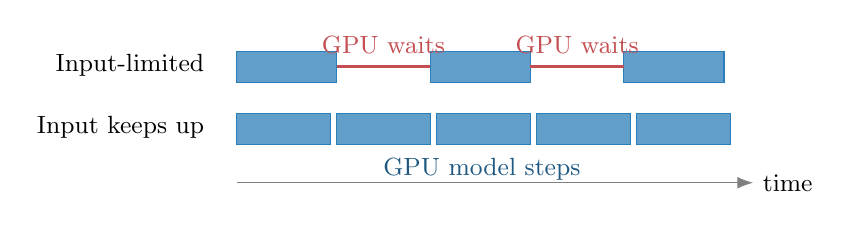
\begin{tikzpicture}[x=0.82cm,y=0.72cm,font=\small]
    \node[anchor=east] at (-0.35,1.35) {Input-limited};
    \node[anchor=east] at (-0.35,0.25) {Input keeps up};
    \foreach \x in {0,3,6} {
      \draw[fill=axblue!75,draw=axblue] (\x,1.05) rectangle +(1.55,0.55);
    }
    \foreach \x in {0,1.55,3.10,4.65,6.20} {
      \draw[fill=axblue!75,draw=axblue] (\x,-0.05) rectangle +(1.45,0.55);
    }
    \draw[waitred,very thick] (1.55,1.325) -- (3,1.325);
    \draw[waitred,very thick] (4.55,1.325) -- (6,1.325);
    \node[waitred,anchor=south] at (2.275,1.38) {GPU waits};
    \node[waitred,anchor=south] at (5.275,1.38) {GPU waits};
    \node[axblue!70!black,anchor=north] at (3.8,-0.12) {GPU model steps};
    \draw[-{Latex[length=2mm]},gray] (0,-0.72) -- (8,-0.72)
      node[anchor=west,black] {time};
  \end{tikzpicture}
  \caption{A slow input path can leave gaps between GPU model steps. The paper
  measures the rate at which the input path produces ready batches. Whether
  that rate changes training time depends on the model's consumption rate.}
  \label{fig:producer-consumer}
\end{figure}

The library decision also depends on transformation coverage. A fast library
cannot execute a transformation it does not provide, and a broad catalog does
not guarantee a fast path for a shared recipe. We therefore answer two questions
separately:

\begin{enumerate}
  \item How many public transformations does each general-purpose Python
  library expose in the maintained coverage census?
  \item For recipes that two implementations both support, which path delivers
  more model-ready batches per second, and how much GPU memory does it allocate?
\end{enumerate}

The resulting recommendation is conditional. On this workload, DALI is the
throughput choice when its recipe set and pipeline architecture fit the project.
\ax{} combines the widest catalog in the census with higher measured throughput
than the evaluated Pillow, TorchVision, and Kornia alternatives on nearly every
shared recipe.

\section{Systems and related work}

The compared libraries make different architectural choices. Pillow exposes
general image operations through a CPU image object~\cite{pillow}. TorchVision
provides tensor and PIL transformations integrated with PyTorch data
loading~\cite{torchvision}. Kornia implements differentiable, batched computer
vision operations on PyTorch tensors and supports accelerator execution
\cite{kornia}. DALI owns the reader, decoder, prefetching, and batched processing
graph, and its mixed decoder can offload JPEG decoding to GPU or dedicated
hardware~\cite{dali}. \ax{} provides CPU augmentation pipelines for images and
related annotations~\cite{albumentationsx}.

These systems do not share one natural execution boundary. Comparing only a
named transform omits decoding, batching, transfer, and normalization. For this
study, every row starts with the same JPEG inventory and ends with the same CUDA
batch contract. Each library retains its native reader, decoder, data type, and
CPU/GPU placement inside that boundary.

\section{Coverage census}

The coverage catalog records 133 public \ax{} operations at version 2.3.7 and
audits whether TorchVision 0.28.0, Kornia 0.8.3, and Pillow 12.3.0 provide a
direct implementation, a partial analogue, or no corresponding public operation.
A partial analogue overlaps in purpose but does not expose the complete
operation contract. Figure~\ref{fig:coverage} counts direct and partial support
separately. This census covers the full public catalog; the execution benchmark
is limited to RGB images.

The coverage advantage has explicit provenance. The author reviewed competing
libraries and deliberately added operations that were missing from \ax{}. The
census measures the current result of that maintenance effort. The 57 execution
recipes form a comparison subset: each recipe is available in at least two
libraries. DALI participates in the execution benchmark, but not in this
class-level census because its public operator reference covers a different graph
and data-loading abstraction.

\begin{figure}[t]
  \centering
  \begin{tikzpicture}
    \begin{axis}[
      xbar stacked,
      width=0.78\textwidth,
      height=5.8cm,
      xmin=0,
      xmax=145,
      xlabel={Public operations (higher is broader)},
      ytick={0,1,2,3},
      yticklabels={Pillow,TorchVision,Kornia,AlbumentationsX},
      bar width=11pt,
      grid=major,
      grid style={gray!15},
      axis line style={gray!45},
      tick style={gray!45},
      tick label style={font=\small},
      label style={font=\small},
      legend style={draw=none,at={(0.98,0.04)},anchor=south east},
    ]
      \addplot[fill=axblue!80,draw=axblue] table[x=direct,y=y] {generated/coverage.dat};
      \addplot[fill=partialorange!80,draw=partialorange] table[x=partial,y=y] {generated/coverage.dat};
      \legend{Direct,Partial}
    \end{axis}
  \end{tikzpicture}
  \caption{The maintained coverage census contains
  \CoverageAlbumentationsX{} \ax{} operations, \CoverageKornia{} Kornia
  operations (including \CoverageKorniaPartial{} partial analogues),
  \CoverageTorchVision{} TorchVision operations (including
  \CoverageTorchVisionPartial{} partial analogues), and \CoveragePillow{}
  Pillow operations. Coverage and execution speed are measured separately.}
  \label{fig:coverage}
\end{figure}

\section{Disk-to-GPU benchmark}

\subsection{Implementations}

The production matrix contains seven implementations. CPU paths perform their
recipe on individual images and transfer a collated batch. GPU-tail paths use
the minimum CPU prefix needed to make differently sized JPEGs collatable, then
run the remaining recipe on the batch. DALI uses its native reader and graph.
Normalize always runs on GPU in \texttt{float16}.

\begin{figure}[t]
  \centering
  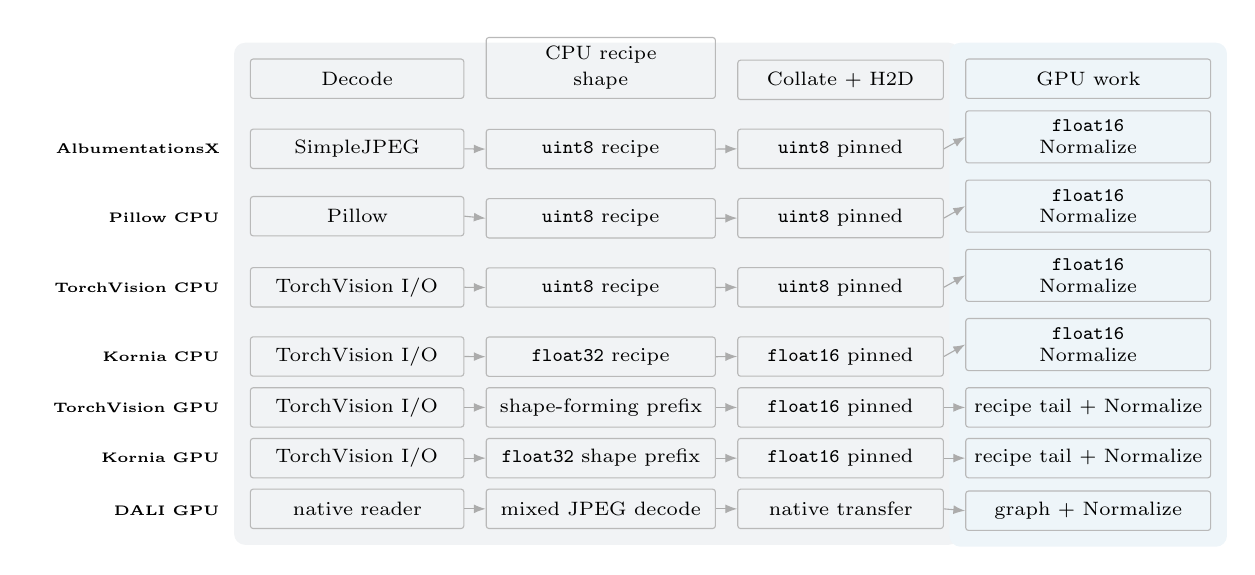
\begin{tikzpicture}[
    stage/.style={draw=gray!55,rounded corners=1pt,minimum height=5mm,align=center,inner xsep=3pt},
    every node/.style={font=\scriptsize},
  ]
    \matrix (paths) [
      matrix of nodes,
      nodes in empty cells,
      row sep=1.3mm,
      column sep=2.7mm,
      column 1/.style={nodes={text width=22mm,align=right,font=\tiny\bfseries}},
      column 2/.style={nodes={stage,text width=25mm}},
      column 3/.style={nodes={stage,text width=27mm}},
      column 4/.style={nodes={stage,text width=24mm}},
      column 5/.style={nodes={stage,text width=29mm}},
    ] {
      & Decode & \shortstack{CPU recipe\\shape} & Collate + H2D & GPU work \\
      AlbumentationsX & SimpleJPEG & \texttt{uint8} recipe & \texttt{uint8} pinned & \shortstack{\texttt{float16}\\Normalize} \\
      Pillow CPU & Pillow & \texttt{uint8} recipe & \texttt{uint8} pinned & \shortstack{\texttt{float16}\\Normalize} \\
      TorchVision CPU & TorchVision I/O & \texttt{uint8} recipe & \texttt{uint8} pinned & \shortstack{\texttt{float16}\\Normalize} \\
      Kornia CPU & TorchVision I/O & \texttt{float32} recipe & \texttt{float16} pinned & \shortstack{\texttt{float16}\\Normalize} \\
      TorchVision GPU & TorchVision I/O & shape-forming prefix & \texttt{float16} pinned & recipe tail + Normalize \\
      Kornia GPU & TorchVision I/O & \texttt{float32} shape prefix & \texttt{float16} pinned & recipe tail + Normalize \\
      DALI GPU & native reader & mixed JPEG decode & native transfer & graph + Normalize \\
    };
    \begin{scope}[on background layer]
      \node[fill=lightgray!65,rounded corners,fit=(paths-1-2)(paths-8-4),inner sep=2mm] {};
      \node[fill=axblue!8,rounded corners,fit=(paths-1-5)(paths-8-5),inner sep=2mm] {};
    \end{scope}
    \foreach \row in {2,...,8} {
      \draw[-{Latex[length=1.5mm]},gray!65] (paths-\row-2.east) -- (paths-\row-3.west);
      \draw[-{Latex[length=1.5mm]},gray!65] (paths-\row-3.east) -- (paths-\row-4.west);
      \draw[-{Latex[length=1.5mm]},gray!65] (paths-\row-4.east) -- (paths-\row-5.west);
    }
  \end{tikzpicture}
  \caption{Measured paths from JPEG to a model-ready CUDA batch. The diagram
  shows placement and transfer dtype; it does not attribute a measured speed
  difference to any single stage.}
  \label{fig:paths}
\end{figure}

The \ax{} path uses SimpleJPEG for decode and a CPU stack built around
Albucore, NumPy, OpenCV, NumKong, StringZilla, and shape/dtype/channel-specific
dispatch, including lookup tables where applicable. The benchmark measures the
combined path. It does not isolate the contribution of a decoder, lookup table,
kernel, or transfer dtype.

\subsection{Workload and measurement}

The input is the first 10,000 \texttt{val/*.JPEG} members of a
SHA-256-verified ImageNet validation archive after lexicographic sorting
\cite{imagenet}. Each seed applies one deterministic random permutation without
replacement, shared by every implementation. The VM reads the selected files
once before measurement, so timed reads normally hit the Linux page cache. File
access and native JPEG decode remain inside the timer; physical cold-disk
bandwidth does not.

All implementations run sequentially on the same Standard
\texttt{g2-standard-16} VM with one NVIDIA L4. Keeping the disk, CPU, and GPU
fixed avoids introducing a hardware change between CPU and GPU implementations.

The catalog contains 57 recipes, each available in at least two libraries.
Parameters are matched manually for practical intent. API names do not imply
pixel-identical outputs: interpolation, random sampling, rounding, and border
handling can differ. \texttt{Resize} means exactly
\texttt{Resize(224) $\rightarrow$ Normalize $\rightarrow$ ToTensor}. Recipes
that require a crop list it explicitly.

Every measured cell has identity
\texttt{(family, implementation, recipe, seed)}. It runs one warm-up batch and
then measures 32 batches, or 8,192 images. The timer covers:

\begin{center}
\texttt{JPEG read/decode $\rightarrow$ recipe $\rightarrow$ collate
$\rightarrow$ pinned H2D $\rightarrow$ GPU tail $\rightarrow$ Normalize
$\rightarrow$ CUDA sync}.
\end{center}

Imports, graph construction, worker startup, and the warm-up batch remain
outside throughput timing. An NVML process-memory monitor starts before pipeline
construction and runs through the final CUDA synchronization. Throughput and
peak GPU memory therefore come from the same pass. Each reported recipe value is
the median over seeds 137, 138, and 139.

\section{Results}

\subsection{The intersection shared by every implementation}

All seven implementations support \CommonRecipeCount{} common recipes.
Figure~\ref{fig:common-results} shows every recipe median and the median across
those recipes. DALI has the highest median throughput at
\CommonSpeedDALIGPU{} images/s. \ax{} follows at
\CommonSpeedAlbumentationsX{} images/s, then TorchVision GPU
(\CommonSpeedTorchVisionGPU{}), TorchVision CPU
(\CommonSpeedTorchVisionCPU{}), Pillow (\CommonSpeedPillowCPU{}), Kornia GPU
(\CommonSpeedKorniaGPU{}), and Kornia CPU (\CommonSpeedKorniaCPU{}).

\begin{figure}[t]
  \centering
  \textbf{(a) Throughput}\par\smallskip
  \begin{tikzpicture}
    \begin{axis}[
      width=0.78\textwidth,
      height=4.7cm,
      xmode=log,
      xmin=15,
      xmax=11000,
      xtick={30,100,300,1000,3000,10000},
      xticklabels={30,100,300,1k,3k,10k},
      xlabel={Images/s (higher is better)},
      ytick={0,1,2,3,4,5,6},
      yticklabels={Kornia CPU,Kornia GPU,Pillow CPU,TorchVision CPU,TorchVision GPU,AlbumentationsX,DALI GPU},
      grid=major,
      grid style={gray!15},
      axis line style={gray!45},
      tick style={gray!45},
      tick label style={font=\small},
      label style={font=\small},
    ]
      \addplot[only marks,mark=*,mark size=1.25pt,gray!55,opacity=0.65]
        table[x=x,y=y] {generated/common-throughput.dat};
      \addplot[only marks,mark=diamond*,mark size=3.2pt,axblue]
        table[x=x,y=y] {generated/common-throughput-medians.dat};
    \end{axis}
  \end{tikzpicture}

  \textbf{(b) Peak process GPU memory}\par\smallskip
  \begin{tikzpicture}
    \begin{axis}[
      width=0.78\textwidth,
      height=4.7cm,
      xmin=1650,
      xmax=2200,
      xtick={1700,1800,1900,2000,2100,2200},
      xlabel={MiB (lower is better)},
      ytick={0,1,2,3,4,5,6},
      yticklabels={Kornia CPU,Kornia GPU,Pillow CPU,TorchVision CPU,TorchVision GPU,AlbumentationsX,DALI GPU},
      grid=major,
      grid style={gray!15},
      axis line style={gray!45},
      tick style={gray!45},
      tick label style={font=\small},
      label style={font=\small},
    ]
      \addplot[only marks,mark=*,mark size=1.25pt,gray!55,opacity=0.65]
        table[x=x,y=y] {generated/common-memory.dat};
      \addplot[only marks,mark=diamond*,mark size=3.2pt,axblue]
        table[x=x,y=y] {generated/common-memory-medians.dat};
    \end{axis}
  \end{tikzpicture}
  \caption{Results on the exact \CommonRecipeCount{}-recipe intersection of all
  seven implementations. Each gray dot is one recipe median across three seeds;
  each blue diamond is the median across recipes. Throughput uses a logarithmic
  axis because individual implementations span more than two orders of
  magnitude on this set. GPU memory is the peak allocation of the input-pipeline
  process, measured in the same pass as throughput.}
  \label{fig:common-results}
\end{figure}

The memory ranking differs from the throughput ranking. Across the common set,
DALI's median peak is \CommonMemoryDALIGPU{} MiB and \ax{} uses
\CommonMemoryAlbumentationsX{} MiB. The GPU-tail paths can allocate more memory
for particular recipes: the largest recipe medians are
\CommonMemoryMaxKorniaGPU{} MiB for Kornia GPU and
\CommonMemoryMaxTorchVisionGPU{} MiB for TorchVision GPU. These values exclude
model parameters, activations, gradients, and optimizer state.

\subsection{Pairwise intersections}

Pairwise comparisons use every recipe shared by \ax{} and the competing
library. For TorchVision and Kornia, the comparison chooses whichever of the
CPU or GPU path is faster for that recipe. This gives each library its strongest
measured result instead of fixing one placement for the whole comparison.

\begin{figure}[t]
  \centering
  \begin{tikzpicture}
    \begin{axis}[
      width=0.88\textwidth,
      height=4.5cm,
      xmode=log,
      xmin=0.3,
      xmax=10,
      xtick={0.5,1,2,4,8},
      xticklabels={0.5,1,2,4,8},
      xlabel={AlbumentationsX throughput / fastest competing path (higher is better)},
      ytick={0,1,2,3},
      yticklabels={Kornia,TorchVision,Pillow,DALI},
      ymin=-0.4,
      ymax=3.4,
      grid=major,
      grid style={gray!15},
      axis line style={gray!45},
      tick style={gray!45},
    ]
      \addplot[black,densely dashed] coordinates {(1,-0.4) (1,3.4)};
      \addplot[only marks,mark=*,mark size=1.4pt,gray!55,opacity=0.65]
        table[x=x,y=y] {generated/pairwise-speedup.dat};
      \addplot[only marks,mark=diamond*,mark size=3.5pt,axblue]
        table[x=x,y=y] {generated/pairwise-speedup-medians.dat};
    \end{axis}
  \end{tikzpicture}
  \caption{Pairwise speed ratios on exact shared recipe sets. Each gray dot is
  one recipe median across three seeds; blue diamonds are medians across recipes.
  The dashed line marks equal throughput. TorchVision and Kornia contribute
  their faster CPU or GPU implementation separately for each recipe.}
  \label{fig:pairwise}
\end{figure}

\ax{} wins every TorchVision comparison, with a median
\PairTorchVisionSpeedup\(\times\) speedup, and
\PairKorniaWins{} of \PairKorniaShared{} Kornia comparisons, with a median
\PairKorniaSpeedup\(\times\) speedup. Kornia GPU is faster for
\texttt{ThinPlateSpline}. \ax{} wins \PairPillowWins{} of
\PairPillowShared{} Pillow comparisons, with a median
\PairPillowSpeedup\(\times\) speedup; Pillow is faster for \texttt{Rotate}.
DALI wins all \PairDALIShared{} shared recipes. Its median advantage is
\PairDALIVsAXSpeedup\(\times\).

At the median of each exact pairwise intersection, \ax{} uses
\PairDALIMemoryMagnitude{} MiB less peak GPU memory than DALI,
\PairPillowMemoryMagnitude{} MiB more than Pillow,
\PairTorchVisionMemoryMagnitude{} MiB more than the selected TorchVision path,
and \PairKorniaMemoryMagnitude{} MiB less than the selected Kornia path.

\FloatBarrier

\section{What the results mean}

The data support two distinct choices. For a project whose augmentation policy
lies within the \PairDALIShared{} measured recipes shared with DALI and whose
stack can adopt DALI's native reader and graph, DALI is the fastest measured
path. It also uses \PairDALIMemoryMagnitude{} MiB more peak GPU memory than
\ax{} at the median of that intersection.

For projects choosing among general Python augmentation libraries, \ax{} offers
the broadest catalog in the maintained census and higher measured throughput on
all \PairTorchVisionShared{} shared TorchVision recipes,
\PairKorniaWins{} of \PairKorniaShared{} Kornia recipes, and
\PairPillowWins{} of \PairPillowShared{} Pillow recipes. The benchmark does not
identify one universal cause. \ax{} combines a native JPEG decoder,
\texttt{uint8} CPU processing and transfer, optimized atomic libraries, and
per-input dispatch; the integrated measurement captures their combined effect.

Input throughput becomes training speed only when the model would otherwise
wait for data. Teams whose GPU is already continuously occupied by model compute
may choose \ax{} for coverage without expecting a shorter epoch. Teams whose
loader cannot keep the model supplied can compare the reported images/s with
their model's batch-consumption rate to estimate whether a library change can
remove the gap.

\section{Limitations}

The study uses one machine type, one L4, one batch size, one worker policy, one
image resolution, and prewarmed local files. The ranking can change with another
CPU/GPU balance, storage system, channel count, video representation, or volume
format. Future 9-channel, video, and volume studies require their own batch sizes,
datasets, recipes, and run identities.

Recipes match practical intent, not exact pixels. Public APIs differ in random
sampling, interpolation, rounding, border rules, and per-image versus per-batch
semantics. The benchmark establishes execution performance for the implemented
recipes; it does not establish numerical equivalence, model accuracy, or
convergence.

Peak process GPU memory is measured without a model. It quantifies augmentation
headroom on the L4 but cannot predict the largest trainable model or batch in a
co-resident training process. The experiment also measures an integrated path,
so it cannot assign a speed difference causally to decode, one transform kernel,
H2D transfer, or normalization.

\clearpage
\appendix

\section{Frozen workload and versions}

\begin{table}[h]
  \centering
  \renewcommand{\arraystretch}{1.18}
  \setlength{\tabcolsep}{5pt}
  \begin{tabularx}{\textwidth}{lY}
    \textbf{Field} & \textbf{Frozen value} \\
    \midrule
    Run & \ProductionRunId; \ProductionCellCount{} validated cells \\
    Input & first 10,000 sorted ImageNet-validation \texttt{val/*.JPEG} files \\
    Output & CUDA \texttt{float16}, BCHW, \(256\times3\times224\times224\) \\
    Timing & one warm-up batch; 32 measured batches (8,192 images) \\
    Seeds & 137, 138, 139 \\
    DataLoader & 15 workers, persistent workers, prefetch factor 2, pinned memory \\
    Hardware & Standard \texttt{g2-standard-16}; one NVIDIA L4 \\
    Software image & CUDA 12.9 Ubuntu 22.04 NVIDIA image dated 30 July 2026 \\
  \end{tabularx}
  \caption{The production run freezes the dataset, recipes, code archive,
  package lock, hardware, and timing boundary.}
  \label{tab:frozen-workload}
\end{table}

\begin{table}[h]
  \centering
  \renewcommand{\arraystretch}{1.18}
  \setlength{\tabcolsep}{5pt}
  \begin{tabular}{ll}
    \textbf{Implementation} & \textbf{Measured version} \\
    \midrule
    AlbumentationsX & 2.4.2 \\
    Pillow & 12.3.0 \\
    TorchVision & 0.28.0+cu130 \\
    Kornia & 0.8.3 \\
    NVIDIA DALI & 2.2.0 \\
  \end{tabular}
  \caption{Library versions recorded in the production cells. The separate
  coverage census uses its explicitly dated AlbumentationsX 2.3.7 catalog.}
  \label{tab:versions}
\end{table}

\FloatBarrier

\section{Reproducibility and diagnostics}

The immutable run record hashes the Git commit, source archive, package lock,
dataset archive, recipe catalog, family configuration, and hardware
configuration. Each successful cell writes throughput and peak process GPU
memory to cloud storage immediately. Resume validates existing cell identity and
runs only missing cells. The completed run contains 759 of 759 expected cells,
with no missing, extra, or wrong-run records.

DALI 2.2.0 emitted 88 \texttt{nvtiff\_cuda\_decoder} initialization messages
while evaluating JPEG inputs. No traceback or exception occurred, and all 66
DALI cells returned the required CUDA output and passed schema and run-identity
validation. The messages are preserved as a runtime diagnostic rather than
silently removed.

The generated values and plot data in this manuscript come from
\texttt{paper/generate\_results.py}. The script decodes every raw cell with the
repository's result validator, reconstructs the expected frozen matrix, refuses
missing or foreign cells, and then writes the LaTeX macros, tables, and plot data.

\section{Recipes shared by all implementations}

\begin{center}
  \begin{tabular}{l}
    % Generated by paper/generate_results.py. Do not edit by hand.
\texttt{RandomCrop224+Affine+Normalize+ToTensor} \\
\texttt{RandomCrop224+Brightness+Normalize+ToTensor} \\
\texttt{RandomCrop224+Contrast+Normalize+ToTensor} \\
\texttt{RandomCrop224+Equalize+Normalize+ToTensor} \\
\texttt{RandomCrop224+GaussianBlur+Normalize+ToTensor} \\
\texttt{RandomCrop224+HorizontalFlip+Normalize+ToTensor} \\
\texttt{RandomCrop224+Normalize+ToTensor} \\
\texttt{RandomCrop224+Rotate+Normalize+ToTensor} \\
\texttt{RandomCrop224+VerticalFlip+Normalize+ToTensor} \\
\texttt{RandomResizedCrop+Normalize+ToTensor} \\
\texttt{Resize224+Normalize+ToTensor} \\

  \end{tabular}
\end{center}

\bibliographystyle{plain}
\bibliography{references}

\end{document}
